%%%%%%%%%%%%%%%%%%%%%%%%%%%%%%%%%%%%%%%%%%%%%%%%%%%%%%%%%%%%%%%%%%
%%%%%%%% ICML 2017 EXAMPLE LATEX SUBMISSION FILE %%%%%%%%%%%%%%%%%
%%%%%%%%%%%%%%%%%%%%%%%%%%%%%%%%%%%%%%%%%%%%%%%%%%%%%%%%%%%%%%%%%%

% Use the following line _only_ if you're still using LaTeX 2.09.
%\documentstyle[icml2017,epsf,natbib]{article}
% If you rely on Latex2e packages, like most moden people use this:
\documentclass{article}

% use Times
\usepackage{times}
% For figures
\usepackage{graphicx} % more modern
%\usepackage{epsfig} % less modern
\usepackage{subfigure} 

% For citations
\usepackage{natbib}

% For algorithms
\usepackage{algorithm}
\usepackage{algorithmic}

% As of 2011, we use the hyperref package to produce hyperlinks in the
% resulting PDF.  If this breaks your system, please commend out the
% following usepackage line and replace \usepackage{icml2017} with
% \usepackage[nohyperref]{icml2017} above.
\usepackage{hyperref}

% Packages hyperref and algorithmic misbehave sometimes.  We can fix
% this with the following command.
\newcommand{\theHalgorithm}{\arabic{algorithm}}

% Employ the following version of the ``usepackage'' statement for
% submitting the draft version of the paper for review.  This will set
% the note in the first column to ``Under review.  Do not distribute.''
%\usepackage{icml2017} 

% Employ this version of the ``usepackage'' statement after the paper has
% been accepted, when creating the final version.  This will set the
% note in the first column to ``Proceedings of the...''
\usepackage[accepted]{icml2017}


% The \icmltitle you define below is probably too long as a header.
% Therefore, a short form for the running title is supplied here:
\icmltitlerunning{Feedback-Gated Rectified Linear Units}

\begin{document} 

\twocolumn[
\icmltitle{Feedback-Gated Rectified Linear Units}

% It is OKAY to include author information, even for blind
% submissions: the style file will automatically remove it for you
% unless you've provided the [accepted] option to the icml2017
% package.

% list of affiliations. the first argument should be a (short)
% identifier you will use later to specify author affiliations
% Academic affiliations should list Department, University, City, Region, Country
% Industry affiliations should list Company, City, Region, Country

% you can specify symbols, otherwise they are numbered in order
% ideally, you should not use this facility. affiliations will be numbered
% in order of appearance and this is the preferred way.
\icmlsetsymbol{equal}{*}

\begin{icmlauthorlist}
\icmlauthor{Marco Kemmerling}{ma}

\end{icmlauthorlist}

\icmlaffiliation{ma}{University of Maastricht, Maastricht, The Netherlands}
%\icmlaffiliation{goo}{Googol ShallowMind, New London, Michigan, USA}
%\icmlaffiliation{ed}{University of Edenborrow, Edenborrow, United Kingdom}

\icmlcorrespondingauthor{Marco Kemmerling}{m.kemmerling@student.maastrichtuniversity.nl}

% You may provide any keywords that you 
% find helpful for describing your paper; these are used to populate 
% the "keywords" metadata in the PDF but will not be shown in the document
\icmlkeywords{boring formatting information, machine learning, ICML}

\vskip 0.3in
]

% this must go after the closing bracket ] following \twocolumn[ ...

% This command actually creates the footnote in the first column
% listing the affiliations and the copyright notice.
% The command takes one argument, which is text to display at the start of the footnote.
% The \icmlEqualContribution command is standard text for equal contribution.
% Remove it (just {}) if you do not need this facility.

%\printAffiliationsAndNotice{}  % leave blank if no need to mention equal contribution
\printAffiliationsAndNotice{} % otherwise use the standard text.

\begin{abstract} 
Feedback connections play a prominent role in the human brain but have not received much attention in artificial neural network research. Here, a biologically inspired feedback mechanism which gates rectified linear units is proposed. On the MNIST dataset, autoencoders with feedback show faster convergence, better performance, and more robustness to noise compared to their counterparts without feedback. Some benefits, although less pronounced and less consistent, can be observed when networks with feedback are applied on the CIFAR-10 dataset.\end{abstract} 

\section{Introduction}
\label{introduction}
The brain has served as inspiration for practical models called artificial neural networks (ANNs) for decades. While these models are usually heavily simplified compared to the brain, they have seen massive success in areas such as computer vision, speech recognition, (...), in recent times. 

Despite successes, it is clear that the average human brain is vastly more powerful than any model used in practice today, and as such it may be useful to investigate how and where exactly the brain and ANNs differ. 

While there is clear evidence of prominent feedback connections in the brain, ANNs have overwhelmingly been designed based on solely the feed forward paradigm. Thus, it is of interested if and how the incorporation of feedback may help artificial models. Further, ANNs with feedback are naturally easier to investigate and manipulate than the real brain and could potentially offer insights into exactly what role this mechanism plays in the brain. 

(maybe tell that ornithology story)

In the remainder of this paper, some neuroscientific background is explored, a specific model of a feedback mechanism is examined and in the following section simplified to be incorporated into artificial models. Then experiments results discussion... 


\section{Neuroscientific Background} 
 
\subsection{Neocortex}
The neocortex, part of the cerebral cortex, is a part of the brain that evolved in mammals comparatively recently. It comprises around 80\% of the human brain \cite{markram2004} and is therefore often speculated to be responsible for the emergence of higher intelligence. 

The most abundant type of neuron in the neocortex are pyramidal neurons, constituting between 70-85\% of cells. In contrast to the remaining neurons in the neocortex, so called interneurons, which are mostly inhibitory, pyramidal neurons are excitatory \cite{defelipe1992}. 

As the name suggests, pyramidal neurons have a cell body roughly shaped like a pyramid, with a base at the bottom and an apex at the top. Pyramidal neurons have two types of dendrites: basal dendrites, originating at the base, and one apical dendrite, originating at the apex. This apical dendrite terminates in what is called the apical tuft, where heavy branching of apical dendrite occurs. \cite{defelipe1992}. 

These apical and basal dendrites are not just differently located, but also serve different functions. Basal dendrites receive regular feedforward input, while the apical tuft dendrites receive feedback input. 

The neocortex appears to have a distinct structure which is characterised by its organisation into layers as well as columns. The columnar organisation is based on the observation that neurons stacked on top of each other tend to be connected and have similar response properties, while only few connections exist between columns. Columns are hence hypothesised to be a basic functional unit in the cortex, although this is somewhat debated in the neuroscience community \cite{goodhill2002}.

The further organisation into six layers was proposed by Brodman in 1909 [citation]. Layers 1 and 6 are of particular interest here. Layer 1 consists of almost no cell bodies, but mostly connections between axons and the apical dendrites of pyramidal neurons \cite{shipp2007}, i.e. is serves as a connection hub for feedback signals. Layer 6 sends signals to neurons in the thalamus which then in turn sends signals to layer 1 neurons in the same column \cite{shipp2007}, i.e. layers 1 and 6 create a loop where feedback is sent from layer 6 and received by layer 1.  
\subsection{Distal Input to Pyramidal Neurons}
As described above, apical tuft dendrites receive feedback input which appears to modulate the gain of the corresponding neuron \cite{larkum2004}. It is hypothesised that this is a way for the cortex to combine an internal representation of the world with external input, i.e. feedback to a neuron may predict whether this particular should be firing and even small feedforward input may lead the neuron to fire as long as the feedback signal is strong \cite{larkum2013cellular}. 

Taking both feedforward and feedback input into account, the firing rate of a neuron can be modelled as follows \cite{larkum2004}:

\begin{equation} 
	\label{eq:neurogain}
	f = g(\mu_S + \alpha \mu_D + \sigma + f\beta(\mu_D)-\theta)
\end{equation}

where $f$ is the firing rate of the neuron, $g$ the gain, $\mu_S$ the average somatic current (i.e. feedforward input), $\mu_D$ the average distal current (i.e. feedback input), $\alpha$ is an attenuation factor, $\sigma$ represents fluctuations in the current, $\theta$ is the firing threshold, and $\beta(\mu_D)$ is an increasing function of the dendritic mean current which saturates for values above some current threshold.  

\section{Feedback-Gated Rectified Linear Units} 
The model described in the previous section serves as a basis to derive an activation function which can replace the common rectified linear unit (ReLU) \cite{nair2010rectified}, i.e. $f(x) = max(0, x)$.  

To arrive at a more practical activation function, $g$ and $\theta$ are dropped from equation \ref{eq:neurogain}, since the threshold is modelled through the bias unit and the gain (i.e. slope) of a ReLU is by definition $1$ and can thus be safely dropped. Dropping the summands $\alpha \mu_D$ and $\sigma$ is less justifiable, but since they do not contribute to the core property of gain increase, they will be disregarded here, arriving at the following simplified relationship: 

\begin{equation}
	f = \mu_S + f\beta(\mu_D)
\end{equation}

Removing $f$ from the right hand side: 
\begin{equation} 
\label{eq:rate1}
	f = \frac{1}{1 - \beta(\mu_D)} \mu_S
\end{equation}

What remains is an exact definition of $\beta(\mu_D)$, which, according to \cite{larkum2004}, is ``an increasing function of the dendritic mean current $\mu$ which saturates for values above 1000pA``. In other words, the function is bounded, i.e. the gain cannot be increased to arbitrarily high values. Accordingly, some maximum value $\beta_{max}$ the function can produce and a threshold value $\eta$ which describes when this maximum is reached need to be defined. 
Assuming a piecewise linear model, $\beta(\mu_D)$ is thus defined as follows: 
\begin{equation}
\label{eq:betafunc}
	\beta(\mu_D) = min \bigg(\frac{\beta_{max}}{\eta} \mu_D, \beta_{max}\bigg)
\end{equation} 

As there are no obvious values to assign to $\beta_{max}$ and $\eta$, they are treated as hyperparameters. Since setting $\beta_{max}$ to 1 results in a division by $0$ and a value of $\beta_{max} > 1$ causes a negative slope, $\beta_{max}$ should be smaller than $1$. 

Plugging equation \ref{eq:betafunc} into equation \ref{eq:rate1} yields: 
\begin{equation}
	f = \frac{1}{1 - min(\frac{\beta_{max}}{\eta} \ \mu_D, \beta_{max})} \ \mu_S 
\end{equation}

Since negative values for $\mu_S$ are not taken account, it is replaced with $max(0, \mu_S)$, i.e. the classic ReLU function: 
\begin{equation}
\label{eq:fgrelu}
		f = \frac{max(0, \mu_S)}{1 - min(\frac{\beta_{max}}{\eta} \ \mu_D, \beta_{max})} 
\end{equation}

\subsection{Feedback-Gated ReLUs in Practice}
The feedback path attempts to mimic the top-down path in the brain. As such, the origin of feedback terminating in a layer should be a layer that is higher in the (feedforward) hierarchy. 

Since feedback from higher layers can only be computed if these higher layers have received feedforward input, at least two time steps are needed to incorporate the modified ReLUs into a network. Concretely, some data, e.g. an image is fed into the network twice, where the first pass enables the computation of feedback which can be utilised in the second pass. 
	Although more than two timesteps are not necessary, it is possible to use an arbitrary number of timesteps, which is examined in section \ref{timesteps}.
	
Any layer that receives feedback requires an additional set of weights to compute $\mu_D$. Specifically each layer $h_i$ with size $n$ receiving feedback from layer $h_j$ with size $m$ introduces $n \times m$ additional parameters.  
	
Dropout \cite{srivastava2014dropout} should be used by dropping out the same units in all passes.  
If e.g. dropout is only applied on the last pass, the remaining units will still receive signals from dropped out units in previous passes.

In convolutional neural networks \cite{lecun1989generalization}, feedback is implemented on a filter-wise basis, i.e. each neuron does not receive its own unique feedback signal, but rather every filter receives a unique feedback signal that is shared between all units belonging to that filter. 


\section{MNIST}
\label{mnist}
GIVE SOME INTRODUCTION TO EXPERIMENT SECTION HERE (SHOULD TIE BACK INTO THE RESEARCH QUESTIONS POSED IN THE INTRODUCTION)

The MNIST dataset is composed of $28 \times 28$ pixel binary images of handwritten digits, split into $60000$ training and $10000$ test instances \cite{lecun2010mnist}. Each image is associated with one of ten classes representing the digits between $0$ and $9$. 

The models used in the following experiments are based on a (non-convolutional) autoencoder with two encoding and two decoding layers. The input layer has dimension $(1\times784)$, the first encoding layer (E1) outputs data of dimension $(1\times392)$, the second (E2) of dimension $(1\times196)$, the first decoding layer (D1) of dimension $(1\times392)$ and the second decoding layer (D2) restores the data back to its original dimension. Except for the final layer, each layer is followed by a ReLU activation. The final layer makes use of a sigmoid activation function. 

First experiments were performed with only a single feedback connection between the first decoder and the first encoder (see figure \ref{fig:autoenc}). 

\begin{figure}
      \centering
      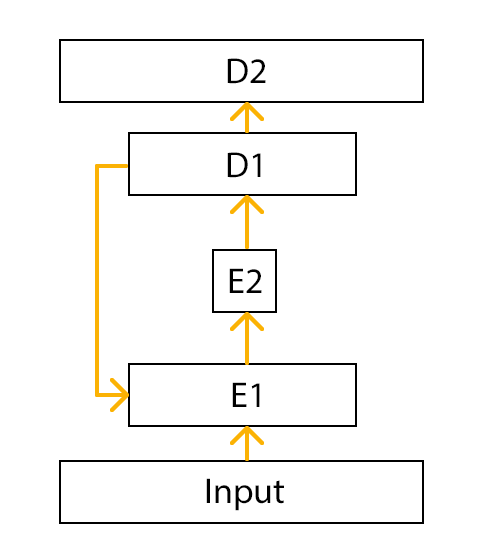
\includegraphics[width=0.5\textwidth,height=5cm,keepaspectratio]{img/AutoEnc.png}
      \caption{Autoencoder with (partial) feedback.}
      \label{fig:autoenc}
  \end{figure}
  
Optimal values for $\eta$ and $\beta_{max}$ were determined by a grid search ($\beta_{max}=0.95, \eta=5$).
 \begin{figure}
      \centering
      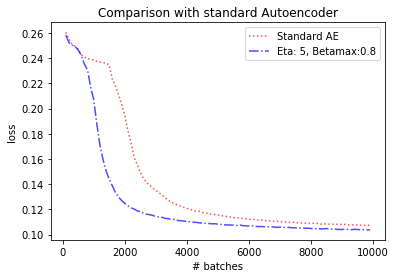
\includegraphics[width=0.5\textwidth,height=5cm,keepaspectratio]{img/fb_vs_nofb.png}
      \caption{Placeholder, make sure to update this figure}
      \label{fig:fbvsnofb}
  \end{figure}
  
To increase the difficulty of the task, the dimension of the second encoding layer is reduced to 10 and the experiment is repeated (this modification will persist in all subsequent experiments).

(results) 

\subsection{More Than Two Timesteps}
\label{timesteps}
While at least two timesteps are required to incorporate feedback, it is not clear whether exactly two timesteps should be used or whether $>2$ timesteps can be beneficial. To examine this, autoencoders with 1, 2, 4, 6, and 8 timesteps are trained. 

The results, depicted in figure \ref{fig:timesteps}, show that more than two timesteps yield no or negligible improvement. This may of course be data and/or task dependent. Since MNIST is a fairly simple dataset (binary images, clear separation of background and foreground, etc.), it is not inconceivable that tasks on other datasets may benefit from more than two timesteps. 




\begin{figure}
      \centering
      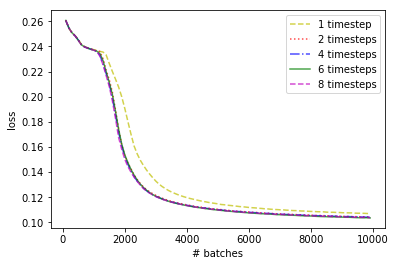
\includegraphics[width=0.5\textwidth,height=5cm,keepaspectratio]{img/timesteps_test.png}
      \caption{Performance with varying numbers of timesteps. Each configuration was trained and evaluated 10 times. The curves shown are the averaged losses on the test set.}
      \label{fig:timesteps}
  \end{figure}
 
 
\subsection{Comprehensive Feedback}
In previous experiments, feedback was only sent from one decoding layer to one encoding layer. Naturally, there are many more opportunities to incorporate feedback. Specifically, in the following, each layer receives feedback from every layer above it.

  \begin{figure}
      \centering
      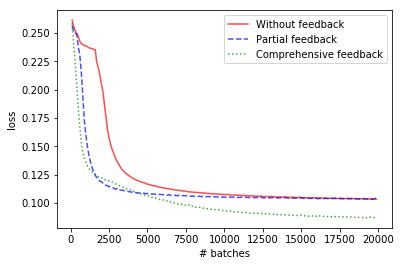
\includegraphics[width=0.5\textwidth,height=5cm,keepaspectratio]{img/fullfb.png}
      \caption{Placeholder, make sure to update this figure}
      \label{fig:fullfeedback}
  \end{figure}
  
  As shown in figure \ref{fig:fullfeedback}, the configuration explained above does not only converge faster than a standard autoencoder, but also settles to a better performance than the model with only partial feedback. 
    
 \subsection{Feedback vs Constant Gain} 
 In an effort to get some understanding how exactly incorporation helps to improve performance, the feedback values computed by a network for all instances of the test set are visualised in a histogram. A distinction is made between feedback and gain, where feedback refers to $\mu_D$ and gain refers to $\frac{1}{1 - min(\frac{\beta_{max}}{\eta} \ (\mu_D), \beta_{max})}$. 
 
 Figure \ref{fig:partialhists} shows the data as collected in the network with a single feedback connection. 
 
 \begin{figure}
      \centering
      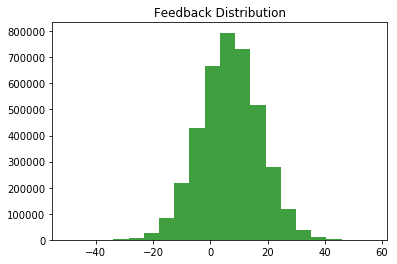
\includegraphics[width=0.5\textwidth,height=5cm,keepaspectratio]{img/constgainpartial.png}
      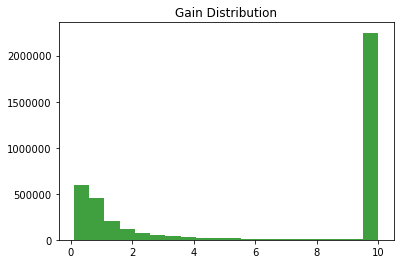
\includegraphics[width=0.5\textwidth,height=5cm,keepaspectratio]{img/constgainpartialgain.png}

      \caption{Distribution of feedback (top) and gain (bottom) values collected in a network with partial feedback over the complete MNIST test set. }
      \label{fig:partialhists}
  \end{figure}
  
  While there are some smaller gain values, the overwhelming majority of values are the maximum gain the network can produce. This raises the question whether there is much benefit to learning feedback or whether it might be similarly beneficial to simply multiply all activation values by a constant. 
  
  This is easily tested by setting the gain of every ReLU in the affected layer to a constant value of 10. 
  \begin{figure}
      \centering
      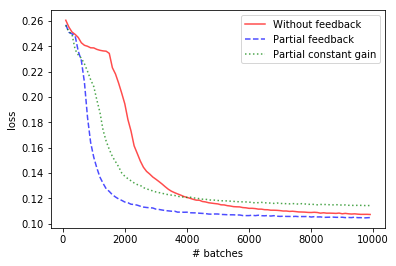
\includegraphics[width=0.5\textwidth,height=5cm,keepaspectratio]{img/constgainpartial_loss.png}
      \caption{Placeholder, make sure to update this figure}
      \label{fig:contgainpartialloss}
  \end{figure}
  
  As can be seen in figure \ref{fig:contgainpartialloss}, this does lead to a steeper loss curve than the standard autoencoder, although not quite as steep as that of the autoencoder with actual learned feedback. Further, the performance after training is completed is worse than that of the standard autoencoder. 
  
  Repeating this same experiment for more than one feedback connection yields to results as illustrated in figure \ref{fig:contgainfullloss}. 
  
  \begin{figure}
      \centering
      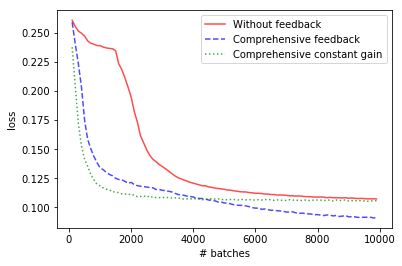
\includegraphics[width=0.5\textwidth,height=5cm,keepaspectratio]{img/constgainfull_loss.png}
      \caption{Placeholder, make sure to update this figure}
      \label{fig:contgainfullloss}
  \end{figure}
  
  In this setup, the simple multiplication by a constant initially converges even faster than the autoencoder with learned feedback. While it does not achieve the same performance as the feedback autoencoder in later stages of training, it is on par with the standard autoencoder's performance. 
  
  Clearly, the effects of feedback cannot be fully explained by this constant gain, but the idea of a constant gain seems to have some merit. 


\subsection{Noisy Activations} 
\label{noisyacts}
While noisy signals are usually not an issue in artificial networks, noise in the brain is very prevalent \cite{Faisal2008}. To see whether feedback makes the model more robust to noise, gaussian noise with zero mean and various standard deviations is added to the (pre-)activations of both the network with feedback and the one without it. The networks are only evaluated with added noise, training is performed without noise. Note that in the network with feedback, noise is added to the activations in both passes.    

		
	\begin{equation}
		h = f(W^T x + b + \mathcal{N}(0,\,\sigma^{2})\,)
	\end{equation}
	
	
	As figure \ref{fig:noiseact} shows, the use of feedback significantly increases the network's robustness to noise. While this is not especially useful for machine learning models, it may be part of the reason why the feedback path exists in the brain. 

	\begin{figure}[H]
      \centering
      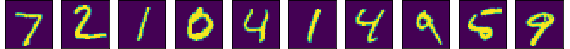
\includegraphics[width=0.45\textwidth,height=5cm,keepaspectratio]{img/actnoise_recs/input.png}
      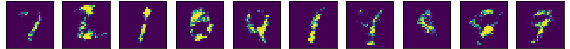
\includegraphics[width=0.45\textwidth,height=5cm,keepaspectratio]{img/actnoise_recs/standardrec.png}
      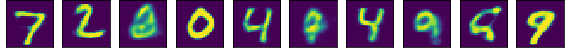
\includegraphics[width=0.45\textwidth,height=5cm,keepaspectratio]{img/actnoise_recs/feedbackrec.png}
      \caption{Gaussian noise with zero mean and standard deviation $\sigma=2.0$ is added to networks with and without feedback. The top row shows input instances to the network, the middle and bottom row show reconstructions of the network without and with feedback (respectively).}
      \label{fig:noiseact}
  \end{figure}
  
  \begin{figure}
      \centering
      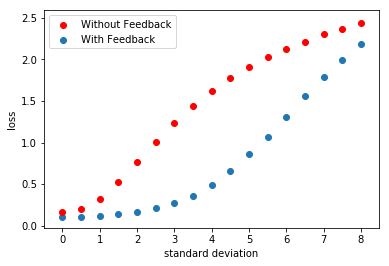
\includegraphics[width=0.5\textwidth,height=5cm,keepaspectratio]{img/actnoise_varstd.png}
      \caption{Gaussian noise with zero mean and varying standard deviations (horizontal) is added to networks with and without feedback. The quality of the reconstruction, as measured by the loss function (vertical axis), with respect to the magnitude of the standard deviation is shown for both networks. }
      \label{fig:noiseact}
  \end{figure}

  
\section{CIFAR-10}
The CIFAR-10 dataset is composed of $32\times32$ pixel colour images of various objects, split into 50000 training and 10000 test instances. Each image belongs to one of the following classes: airplane, automobile, bird, cat, deer, dog, frog, horse, ship, truck \cite{krizhevsky2014cifar}. 

\subsection{Autoencoder}
\label{cifarae}
Similarly to the MNIST experiments, an autoencoder is trained on the CIFAR-10 dataset. Again, the architecture consists of two encoding and two decoding layers. Contrary to MNIST, the encoding/decoding layers used here are convolutional/transposed convolutional layers with 16 $5 \times 5$ filters. 

While the autoencoder with feedback clearly performs better than the one without it, the difference between the two is not as pronounced as it is in the MNIST experiments.   

Curiously, if batch normalisation \cite{ioffe2015batch} is used after the activation functions, feedback cannot improve on the performance of the standard autoencoder. This may suggest that somehow feedback and batch normalisation are interacting in such a way that the feedback is rendered ineffective. 

\begin{figure}
      \centering
      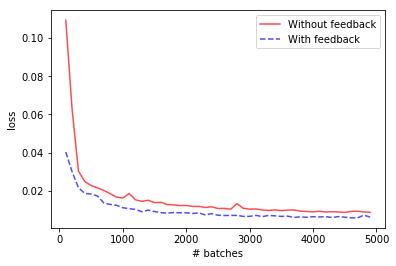
\includegraphics[width=0.5\textwidth,height=5cm,keepaspectratio]{img/cifar_auto_test_loss.png}
      \caption{Test set loss of autoencoders with and without feedback on the CIFAR-10 dataset. Neither model makes use of batch normalisation. }
      \label{fig:cifarauto}
  \end{figure}
  
  \begin{figure}
      \centering
      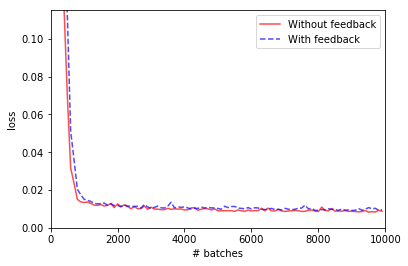
\includegraphics[width=0.5\textwidth,height=5cm,keepaspectratio]{img/cifar_auto_batch_test_loss.png}
      \caption{Test set loss of autoencoders with and without feedback on the CIFAR-10 dataset. Both models make use of batch normalisation. }
      \label{fig:cifarautobatch}
  \end{figure}

\subsection{Noisy Activations}
The experiment from section \ref{noisyacts} is repeated on the CIFAR-10 dataset. The network employed is the autoencoder without batch normalisation from the previous experiment. 

Since feedback increased the robustness to noise in the MNIST autoencoder, the same behaviour would be expected here. However, as apparent in figure \ref{fig:cifarnoise}, the network with feedback is much more sensitive to (even small amounts of) noise than the one without feedback. 

compounding effect   

\begin{figure}
      \centering
      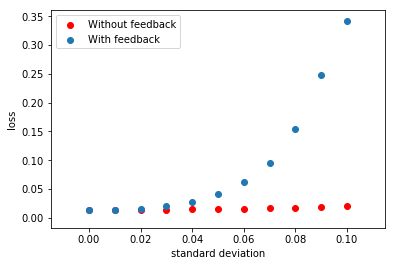
\includegraphics[width=0.5\textwidth,height=5cm,keepaspectratio]{img/cifar_actnoise.png}
      \caption{Gaussian noise with zero mean and varying standard deviations is added to the CIFAR-10 autoencoders with and without feedback. Although this is not apparent due to the scale of the plot, the data for the network without feedback follows a similar shape to the one with feedback.}
      \label{fig:cifarnoise}
  \end{figure}

\subsection{Classification} 
Classification on the CIFAR-10 dataset is performed using a convolutional neural network. The network consists of two convolutional layers with 64 filters of size $5 \times 5$, each followed by a max pooling \cite{zhou1988computation} layer with a $2\times2$ window and a stride of $2$. The convolution  and pooling layers are followed by a fully connected layer (200 units) and a softmax \cite{bridle1990probabilistic} layer. 
Batch normalisation is applied after the pooling layers and dropout with a rate of $0.5$ is applied after the pooling and the fully connected layers. 

To test whether feedback can improve classification performance, the network is trained with and without feedback. Figure \ref{fig:cifarclass} shows only a marginal performance difference between the two networks, with the feedback network being slightly better. 

Note that the network employed here makes use of batch normalisation, which, as shown in the previous section, may be problematic in combination with feedback. Whether this is the case here is not clear, since this particular network will not converge when batch normalisation is disabled (be it with or without feedback). 

\begin{figure}
      \centering
      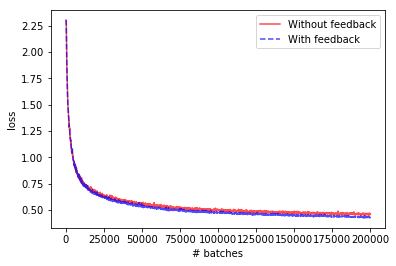
\includegraphics[width=0.5\textwidth,height=5cm,keepaspectratio]{img/cifar_class_test_loss.png}
      \caption{Classification loss on the CIFAR-10 test set. The training time of 200000 batches corresponds to 512 epochs.}
      \label{fig:cifarclass}
  \end{figure}
  
\section{Conclusion}
tell them what you told them 

The feedback mechanism presented here is able to improve performance of conventional networks both in terms of convergence speed and convergence value in certain cases. The effectiveness of the mechanism is inconsistent across different datasets, with ...
This allows two conclusions: (1) the effectiveness of the mechanism is data-dependent, i.e. it may be leveraging the highly regular structure of the MNIST dataset, ... , or (2) the implementation of the mechanism in the CIFAR-10 experiments is not .... Notably, in convolutional networks, feedback is given on a filter-wise basis, which may be too simplistic.  


Noise


Section \ref{cifarae} suggests that there may be an (unfavourable) interaction between the feedback mechanism and batch normalisation. Investigating why this is the case may shed further light on how the feedback works and what role it fulfils. 



suggest future work: relationship feedback batchnorm 

multi modal 


\bibliography{example_paper}
\bibliographystyle{icml2017}

\newpage
\clearpage

\section{Appendix}

\subsection{Hyperparameter Tuning} 
As mention in section \ref{mnist}, optimal values for $\beta_{max}$ and $\eta$ are determined by a grid search. The initial grid is defined by $\eta = [5, 10, 15, \dots, 50]$ and $\beta_{max} = [0.1, 0.2, \dots, 0.8]$. 

The highest value for $\beta_{max} \ (0.8)$ consistently shows the best performance regardless of $\eta$'s values, as exemplified by figure \ref{fig:hyper1}. Note that a high constant value of $\eta$ with varying values of $\beta_{max}$ will generally lead to less spread between the loss curves, since the activation function will be more sensitive to $\beta_{max}$ when $\eta$ is low. 

\begin{figure}[H]
      \centering
      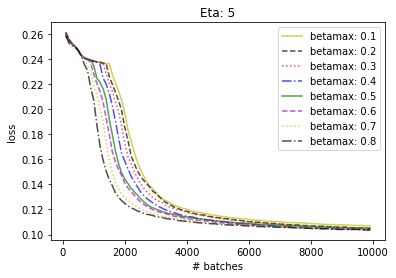
\includegraphics[width=0.5\textwidth,height=5cm,keepaspectratio]{img/appendix/hyper/eta5.png}
      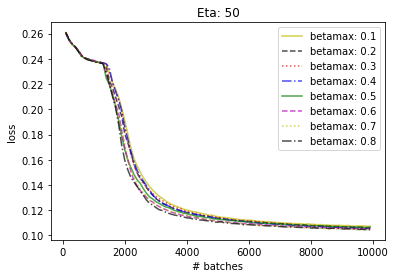
\includegraphics[width=0.5\textwidth,height=5cm,keepaspectratio]{img/appendix/hyper/eta50.png}
      \caption{Top: first pass, bottom: second pass}
      \label{fig:hyper1}
  \end{figure}

While higher values of $\beta_{max}$ lead to better performance, the inverse relationship can be seen with $\eta$, i.e. lower values of $\eta$ lead to better performance. This is illustrated in figure \ref{fig:hyper2}.  

\begin{figure}[H]
      \centering
      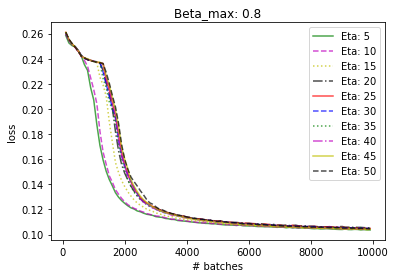
\includegraphics[width=0.5\textwidth,height=5cm,keepaspectratio]{img/appendix/hyper/betamax08.png}
      
      \caption{Top: first pass, bottom: second pass}
      \label{fig:hyper2}
 \end{figure}
 
A second grid search with $\eta = [1, 2, 3, 4, 5], \beta_{max} = [0.8, 0.85, 0.9, 0.95]$ is performed to determine whether even lower/higher values can further improve performance. Indeed, increasing $\beta_{max}$ to $0.95$ leads to better performance, but further decreasing $\eta$ is not advantegeous. 

\subsection{Visualising Activations} 
\begin{figure}
      \centering
      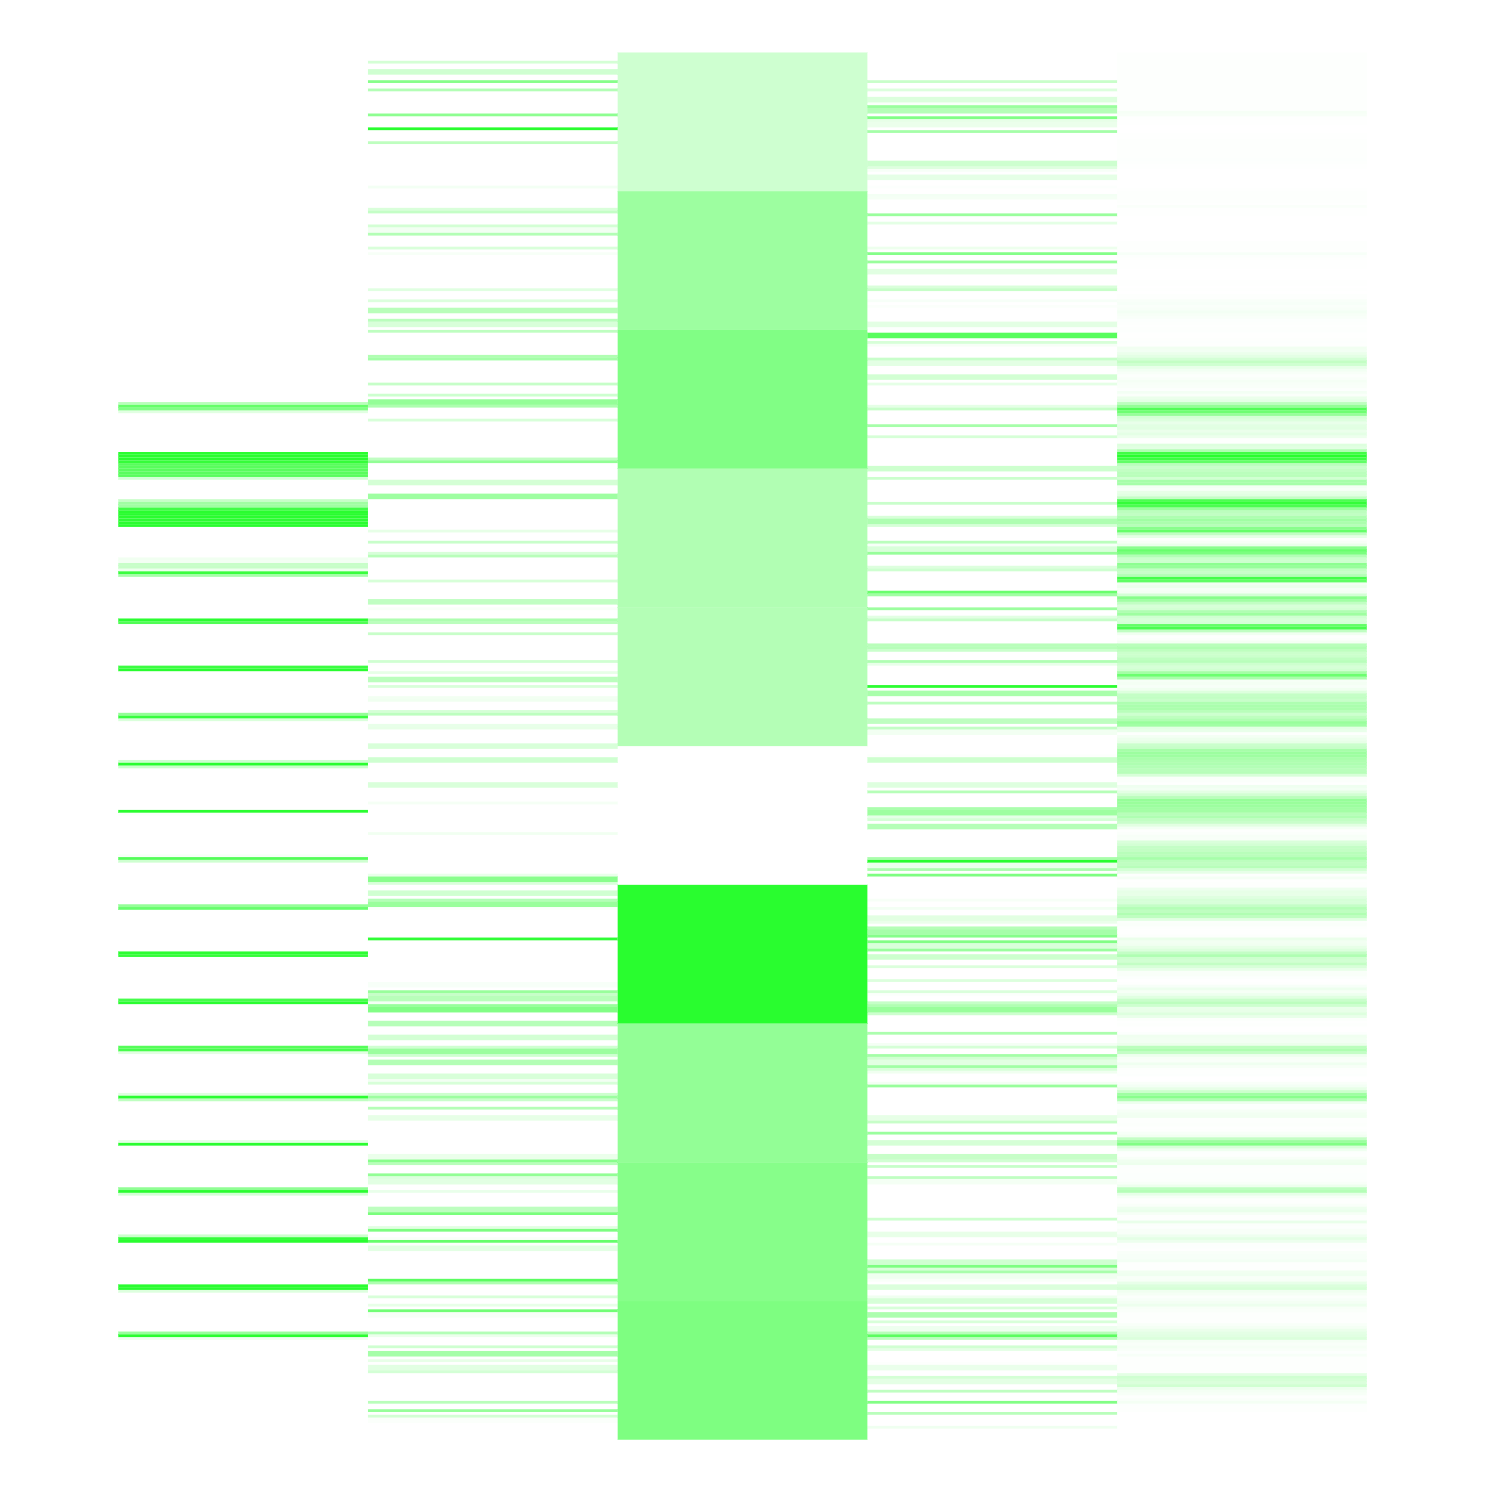
\includegraphics[width=0.5\textwidth,keepaspectratio]{img/appendix/actvis/firstpass.png}
      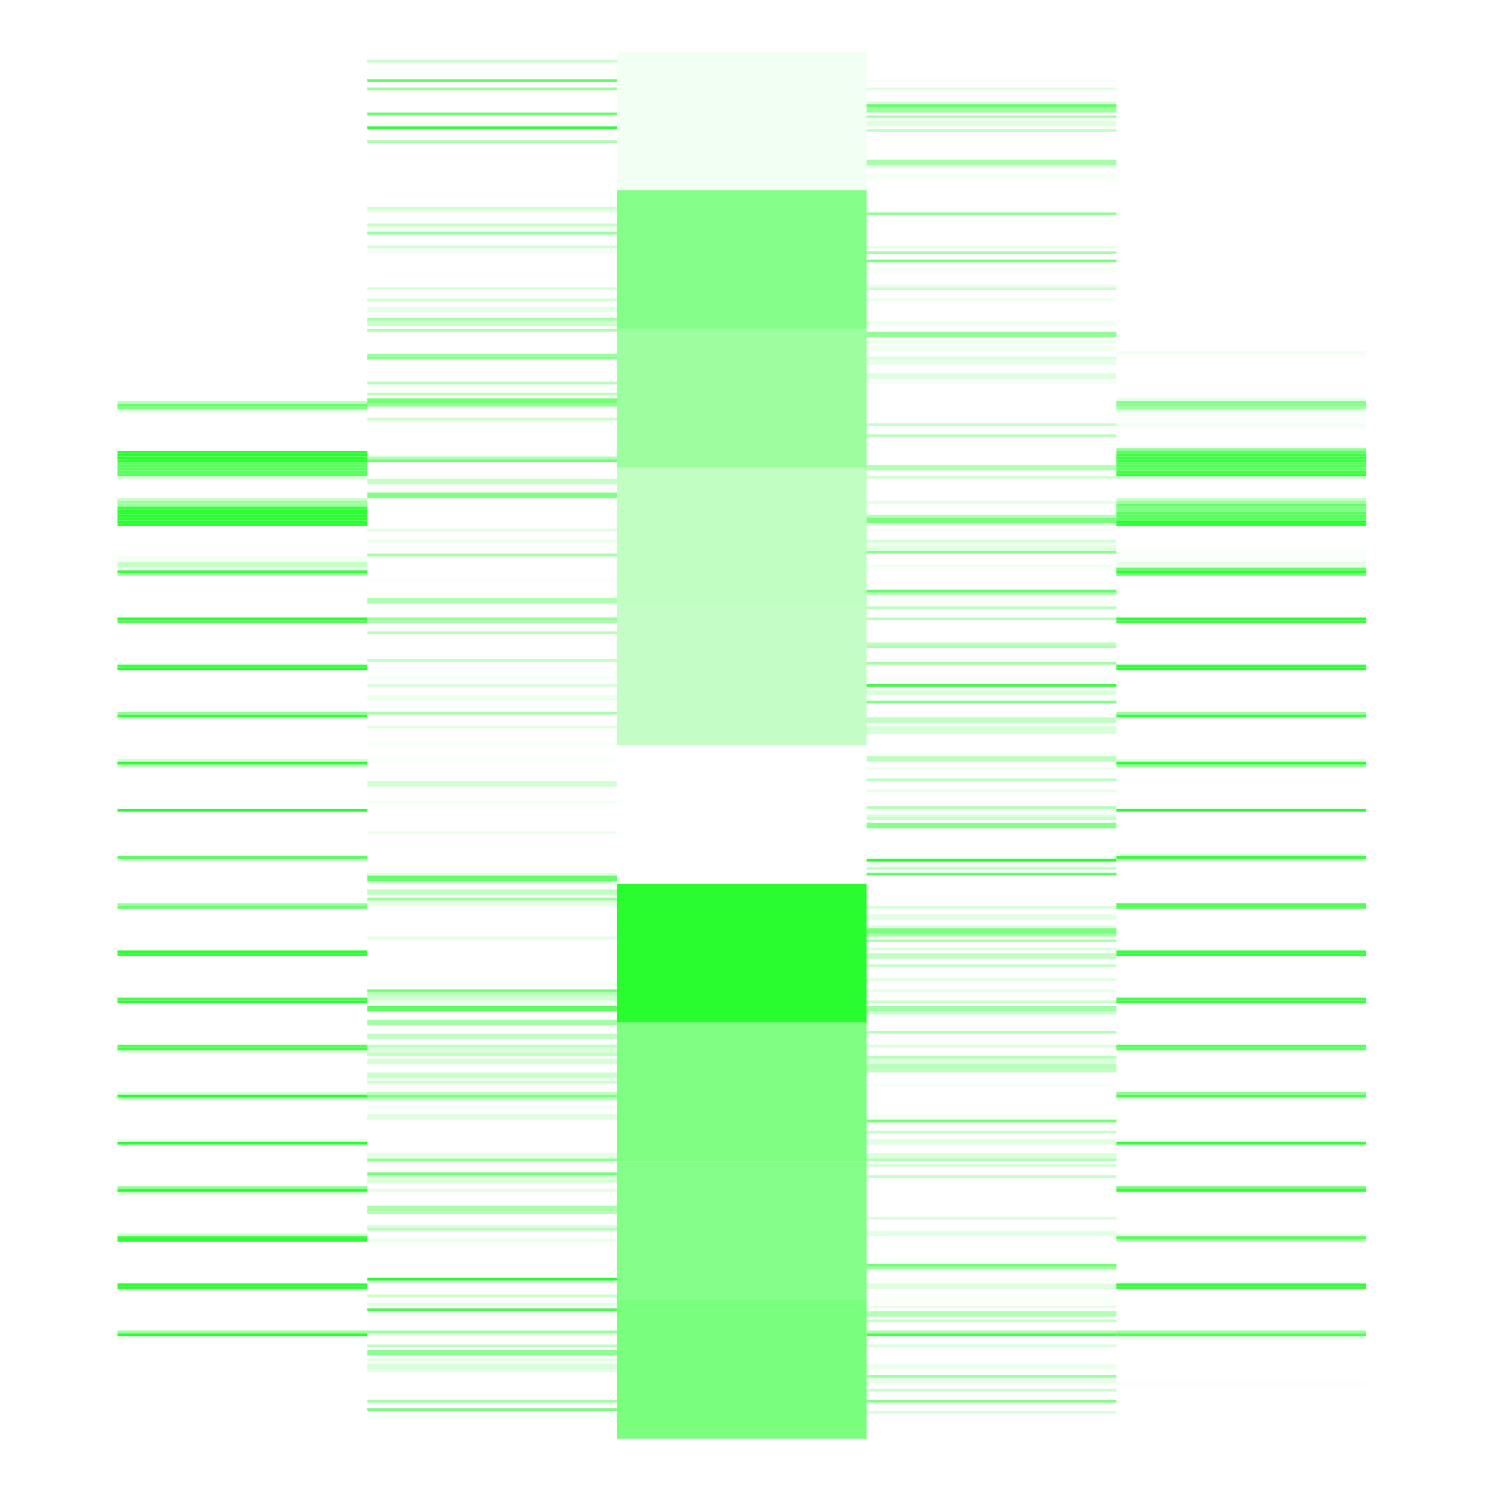
\includegraphics[width=0.5\textwidth,keepaspectratio]{img/appendix/actvis/secondpass.png}
      \caption{Top: first pass, bottom: second pass}
      \label{fig:actvis}
  \end{figure}



\subsection{Feedback-Controlled Threshold} 
Equation \ref{eq:neurogain} describes not only gain modulation through feedback, but also an adjustment of the activation functions threshold, i.e. $\alpha \mu_D$ is one of the terms in the summation. While gain modulation is the main property of interest in this paper, it is conceivable that the change in threshold plays a significant part in this mechanism as well. 

Incorporating this threshold mechanism into equation \ref{eq:fgrelu} leads to: 
\begin{equation}
	f = \frac{max(0, \mu_S + \alpha \mu_D)}{1 - min(\frac{\beta_{max}}{\eta} \ \mu_D, \beta_{max})} 
\end{equation}

where $\alpha$ is a parameter to be learned by the network. While $\alpha$ could also be set to a constant (tuned) value, prior experiments suggest that it is beneficial to let the network adjust $alpha$ during the course of training. 

As can be seen in figure \ref{fig:threshold}, the added threshold mechanism is not able to improve upon the network implementing the gain mechanism. Although the models with feedback-controlled threshold both perform better than the standard autoencoder, the model with only gain and no threshold mechanism still has the overall best performance. 

\begin{figure}[H]
      \centering
      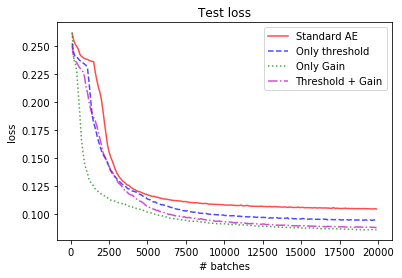
\includegraphics[width=0.5\textwidth,height=5cm,keepaspectratio]{img/appendix/threshold/threshold_test.png}
            \caption{Performance of the standard autoencoder, an autoencoder with feedback-controlled threshold, an autoencoder with feedback-controlled gain, and an autoencoder with both feedback-controlled threshold and gain on the MNIST test set.}
      \label{fig:threshold}
  \end{figure}

\subsection{T-SNE} 
\begin{figure}[H]
      \centering
      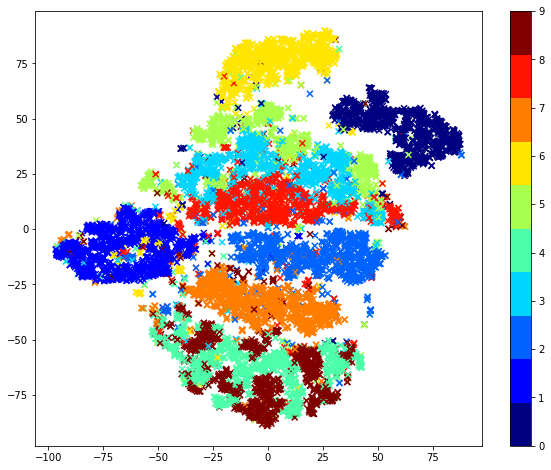
\includegraphics[width=0.5\textwidth,height=5cm,keepaspectratio]{img/appendix/mnist_tsne/firstpass.png}
      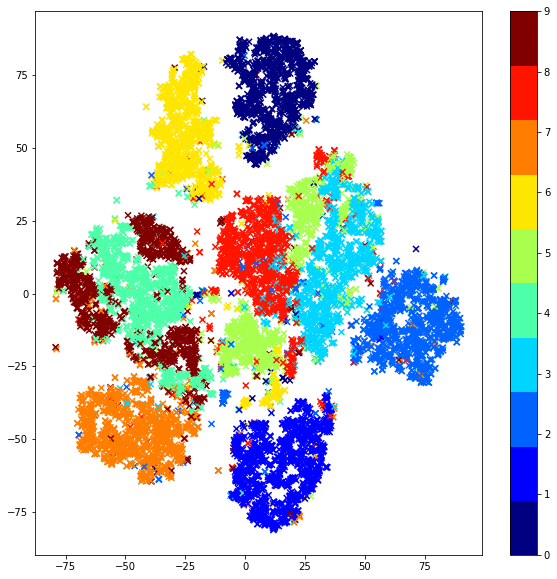
\includegraphics[width=0.5\textwidth,height=5cm,keepaspectratio]{img/appendix/mnist_tsne/secondpass.png}
      \caption{T-SNE visualisation of the second encoding layer of the autoencoder over the whole MNIST test set. Top: first pass, bottom: second pass}
      \label{fig:tsne}
  \end{figure}
  
  \begin{figure}[H]
      \centering
      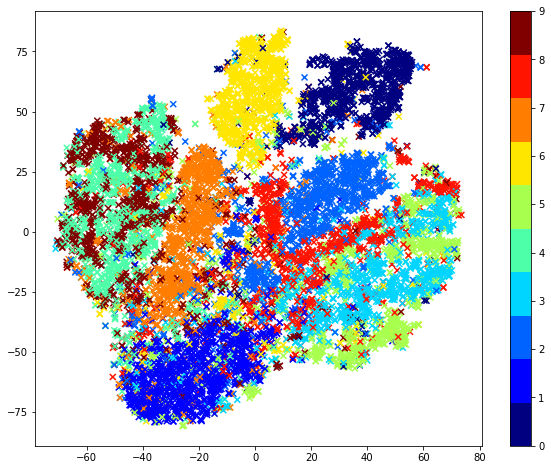
\includegraphics[width=0.5\textwidth,height=5cm,keepaspectratio]{img/appendix/mnist_tsne/noisefirstpass.png}
      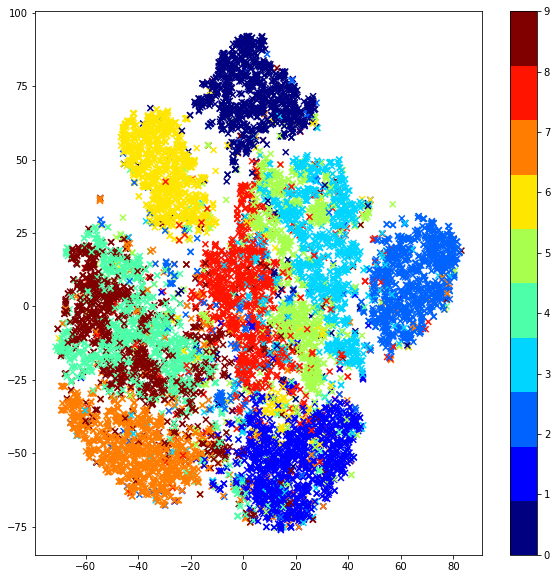
\includegraphics[width=0.5\textwidth,height=5cm,keepaspectratio]{img/appendix/mnist_tsne/noisesecondpass.png}
      \caption{T-SNE visualisation of the second encoding layer of the autoencoder over the whole MNIST test set. Top: first pass, bottom: second pass}
      \label{fig:tsnenoise}
  \end{figure}

  
  
  
 \subsection{Input With Reduced Contrast}
Images with reduced contrast are presented to the trained (on regular contrast images) network, to see if the second pass can reconstruct an image that is more akin to a regular contrast image. To reduce the contrast, each pixel of the image is multiplied by some contrast factor $0 \leq c \leq 1$. 

Figure \ref{fig:contrastdiff} shows the absolute difference in mean pixel value between the first and second pass reconstructions for a number of different contrast factors. A high contrast input image leads to a larger difference in mean pixel value, while a low contrast image leads to a smaller difference between first and second pass reconstructions. 




\begin{figure}[H]
      \centering
      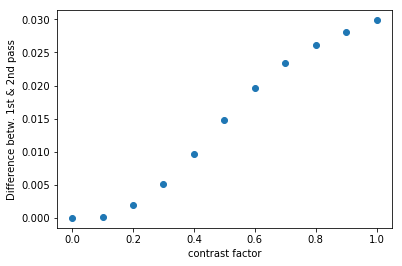
\includegraphics[width=0.5\textwidth,height=5cm,keepaspectratio]{img/appendix/contrast/diff.png}
            \caption{Absolute difference in mean pixel value between first and second pass reconstructions as a function of different contrast factors (from $0.0$ to $1.0$ in $0.1$ increments). A contrast factor of $1.0$ corresponds to no reduction in contrast, while a contrast factor of $0.0$ means the input images are entirely black.}
      \label{fig:contrastdiff}
  \end{figure}
  
  
  \begin{figure}
      \centering
      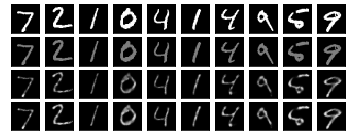
\includegraphics[width=0.5\textwidth,height=5cm,keepaspectratio]{img/appendix/contrast/contrastrec.png}
            \caption{From top to bottom: original image, contrast reduced image, first pass reconstruction, second pass reconstruction. The contrast reduced image was produced by multiplying the original image with a contrast factor of $0.5$, i.e. each pixel in the contrast reduced image has values in the range $[0.0, 0.5]$ instead of $[0.0, 1.0]$}
      \label{fig:contrastdiff}
  \end{figure}

  
  
 \subsection{Reflections} 
 
 material learned: got more comfortable with neural nets (theory - practice divide), initialisations, batchnorm, data normalisation 
 
 

\end{document} 


% This document was modified from the file originally made available by
% Pat Langley and Andrea Danyluk for ICML-2K. This version was
% created by Lise Getoor and Tobias Scheffer, it was slightly modified  
% from the 2010 version by Thorsten Joachims & Johannes Fuernkranz, 
% slightly modified from the 2009 version by Kiri Wagstaff and 
% Sam Roweis's 2008 version, which is slightly modified from 
% Prasad Tadepalli's 2007 version which is a lightly 
% changed version of the previous year's version by Andrew Moore, 
% which was in turn edited from those of Kristian Kersting and 
% Codrina Lauth. Alex Smola contributed to the algorithmic style files.  
